%
% Anlagendesign
%
% @version 1.0
% @author dmayer
% @created 29. Dezember 2015

\setchapterpreamble[o]{%
\dictum[--- \textsc{Charles Eames}]{\Gun Design is the appropriate combination of materials in order to solve a problem. \Gob}}
\renewcommand{\chapterheadstartvskip}{\vspace*{2cm}}

\chapter{Anlagendesign}
\label{chap:anlagendesign}

\renewcommand{\chapterheadstartvskip}{\vspace*{-0.5cm}}

In diesem Kapitel werden zunächst die Anforderungen an eine Anlage zur Raumtemperaturregelung für den Betrieb mit Modellprädiktiver Regelung analysiert. Weiterhin werden die anlagenbezogenen Vorgaben und Rahmenbedingungen von Seiten der Hochschule Karlsruhe spezifiziert und ausgeführt. Daraus wird eine Idee abgeleitet, die anschließend zu einem Konzept weiterentwickelt und in ein konkretes Anlagendesign umgesetzt wird. Dabei werden die einzelnen Anlagenteile und deren Funktionsweisen näher beschrieben und auf die realen Einsatzbedingungen ausgelegt. 
%Unzufrieden mit letztem Satz.
Abschließend wird die Realisierung und die bei der Installation aufgetretenen Besonderheiten der Anlage beschrieben.


\section{Analyse der Anforderungen und Rahmenbedingungen}
\label{sec:anforderungen}

Um die Anforderungen an eine gewünschte Anlage zu bestimmen, muss zunächst der Zweck und die Einsatzziele der Anlage untersucht werden. In Kapitel \ref{sec:motivation} wurde bereits darauf hingewiesen, dass es die Vorgabe von Seiten der Hochschule war, die Einsatzziele in Einklang und komplementär zu der bisherigen Forschung wählen. Daher wurden im Dialog mit den Projektverantwortlichen der Hochschule Karlsruhe für die Forschung von MPC in solaren Anwendungen, in Person von Herrn \textsc{Adrian Bürger} und \textsc{Markus Bohlayer}, gemeinsam konkrete Einsatzziele für eine --wie in forsch frage gewünschte-- Anlage erarbeitet. Konkret werden mit dem Einsatz der Anlage die folgende Ziele verfolgt:
 
\begin{itemize}
	\item Die Einarbeitung in die Thematiken Modellbildung, Kommunikation technischer Systeme und Modellprädiktive Regelung soll durch eine praktisches Anwendung unterstützt werden.
	\item Es soll Knowhow bei der Kommunikation technischer Systeme aufgebaut werden, insbesondere im Umgang mit der Software, der Hardware und zahlreichen Schnittstellen.
	\item Die Anlage soll eine hohe Funktionalität, also möglichst wartungsarm, und eine hohe Robustheit gegenüber Fehlern und Beschädigungen besitzen, da bei der Einarbeitung eine erhöhte Wahrscheinlichkeit der Fehlbedienung besteht und Schäden dadurch vermieden werden sollen.
	\item Es soll ein Vergleich verschiedener Regelungsmethodiken beim Einsatz von Modellprädiktiver Regelung ermöglicht werden.
	\item Außerdem soll ein Vergleich von Ergebnissen ermöglicht werden, bei der Variation von Steuerungsparametern sowie beim Einsatz verschiedener Steuerungs- und Regelungsalgorithmen.
\end{itemize}

Zusammenfassend wurde festgehalten, dass die Anlage als Forschungsumgebung für Entwicklungs-, Test- und Anwendungszwecke für verschiedene Steuerungen dienen soll.

%Here we go

Weiterhin wurden von Seiten der Hochschule Karlsruhe, in den Person von Frau Professor \textsc{Angelika Altmann-Dieses}, Herrn Professor \textsc{Marco Braun} und Herrn \textsc{Adrian Bürger}, weitere Rahmenbedingungen vorgegeben:
\begin{itemize}
	\item Raum für Labor
	\item Minimaler baulicher und finanzieller Aufwand
	\item Modbus Kommunikationstechnologie
	% EVTL fehlt noch was
\end{itemize}


Aus den Einsatzzielen und Rahmenbedingungen lassen sich konkrete Anforderungen ableiten, die in Tabelle \ref{tab:anforderungen_umgebung} zusammengefasst sind.

% Hier gehts weiter mit der Tabelle

\begin{table}[H]
\centering
\small
\renewcommand{\arraystretch}{1.3}
\begin{tabularx}{1\textwidth}{m{0.35\textwidth}m{0.58\textwidth}}

\toprule

\textbf{Einsatzziele} & \textbf{Anforderungen} \\

\cmidrule[0.5pt](r{0.25em}){1-1} 
\cmidrule[0.5pt](l{0.25em}){2-2}

Einarbeitung in die Thematiken	& \multirow{2}{\hsize}{Komplexität erwünscht, allerdings nicht zu hoch}  \\

\cmidrule[0.1pt](lr{2em}){1-1} 

Knowhow Technische Kommunikation							&					\\

\cmidrule[0.5pt](r{0.25em}){1-1} 
\cmidrule[0.5pt](l{0.25em}){2-2}

Vergleich von Ergebnissen		& Schnell und einfach messbare Reaktionen      \\
\cmidrule[0.5pt](r{0.25em}){1-1} 
\cmidrule[0.5pt](l{0.25em}){2-2}

\multirow{2}{\hsize}{Hohe Funktionalität und Robustheit} & Einfache Anwendung mit geringer Störanfälligkeit\\
\cmidrule[0.1pt](lr{2em}){2-2} 

 & Einfache und robuste Einzelkomponenten \\
 
\cmidrule[0.5pt](r{0.25em}){1-1} 
\cmidrule[0.5pt](l{0.25em}){2-2}

Minimaler finanzieller und baulicher Aufwand & \\

\cmidrule[0.5pt](r{0.25em}){1-1} 
\cmidrule[0.5pt](l{0.25em}){2-2}

& Einsatz der Modbus Kommunikationstechnologie \\

\bottomrule
\end{tabularx}
\caption{Übersetzung der Ziele in Anforderungen der Anlage}
\label{tab:anforderungen_umgebung}
\end{table}


Um die Einarbeitung zu vereinfachen sollte die Anlage möglichst wenig Komplexität aufweisen, um die Zusammenhänge und Wechselwirkung zwischen den einzelnen Gebieten und Komponenten möglichst einfach begreifbar zu machen. Da jedoch auch Erfahrungen gesammelt werden sollen, wird ein bestimmtes Maß an Komplexität vorausgesetzt, da diese mit einer wachsenden Zahl von Schnittstellen, verschiedener Soft- und Hardware einhergeht. Dadurch ergibt sich die Forderung nach einem Kompromiss zwischen Verständlichkeit und Komplexität, weshalb ein bestimmtes Maß an Komplexität erwünscht ist.
Das einfache Vergleichen von Ergebnissen soll dadurch ermöglicht werden, dass die Reaktionen/Ergebnisse/Messungen schnell und einfach zu messen sind. Das bedeutet konkret, dass die Anlage zum einen \Gun schnell\Gob eine Reaktion auf Steuerungsimpulse zeigen soll. Zum anderen soll die Reaktion einfach, dass heißt ohne großen technischen und monetären Aufwand und möglichst direkt, messbar sein. Die letzte, sehr wichtige, abgeleitete Anforderung ist eine hohe Funktionalität, um Fehlerquellen außerhalb der Forschung auszuschließen und damit die wissenschaftliche Arbeit zu erleichtern. Entsprechend wird auch eine Robustheit gegenüber Fehlern gefordert, da bei Testeinsätzen von Steuerungen sehr wahrscheinlich auch Fehler passieren sich einstellen und diese keine Schaden an der Anlage verursachen sollen.
Eine weitere Anforderung, unabhängig von den Einsatzzielen oder den technischen Eigenschaften wurde von Seiten der Hochschule vorgegeben: Die Anlage soll mit einem möglichst geringen finanziellen und baulichen Aufwand verbunden sein.


IDEE vielleicht
Trotz einer Vielzahl von technischen Anwendungen, die sich für den im vorangegangenen Kapitel beschriebenen Zweck und dessen Anforderungen eignen, qualifiziert sich  sich besonders eine dafür: Die Steuerung einer Raumtemperatur.


\section{Das Konzept der Anlage}

Trotz einer Vielzahl von technischen Anwendungen, die sich für den im vorangegangenen Kapitel beschriebenen Zweck und dessen Anforderungen eignen, qualifiziert sich  sich besonders eine dafür: Die Steuerung einer Raumtemperatur.

Diese ist mit schnellen als auch einfachen Messungen ohne großen technischen Aufwand verbunden.
, sowie deren Komplexität noch überschaubar ist und mit wenig finanziellem Aufwand verbunden ist. Dadurch ergeben sich zwei potentielle technische Anwendungen: Zum einen die Klimatisierung eines Raumes und zum anderen die Beheizung eines Raumes. Beide weisen ein passendes Maß an Komplexität aufweisen und sich auf Grund ihrer Eigenschaften hervorragend für den Einsatz mit \acrlong{mpc} eignen. Da sich die Raumheizung jedoch mit weniger baulichem und finanziellem Aufwand realisieren lies, wurde letztendlich entschieden diese konkrete Anwendung zum Einsatz zu bringen.


Die Idee der Anlage ist, es mit möglichst wenig Aufwand und Komplexität ermöglichen im ersten Schritt die Raumtemperatur zu erfassen und im nächsten Schritt die Raumtemperatur durch Beheizung zu steuern. Der Bedarf an Komponenten hierfür lässt sich grob in drei verschiedene Gruppen gliedern. Zum einen in die Sensoren zur Ermittlung des Zustandes innerhalb des Raums, der Aktorik zur Beeinflussung des Raumzustandes und einem logischen Controller der die Steuerung der Sensorik und Aktorik übernimmt.
Um den Zustand im Raum zu bestimmen, werden zunächst also Raumtemperatursensoren benötigt. Des Weiteren muss für die Steuerung auch der Zustand der Heizung erfassbar sein, was durch Temperatursensoren am Ein- und Ausgang der Heizung und einen Durchflusssensor überwacht werden soll.
Um den Zustand im Raum beeinflussen zu können, soll der Heizkörper im Raum über einen Aktor am Ventil des Heizkörpers gesteuert werden.
Der logische Controller soll im Rahmen von \acrlong{mpc} Optimalsteuerungspläne berechnen, wofür aureichende Rechenkapazität zur Verfügung stehen muss -- da Optimierung gradientenbasiert erfolgt -- weshalb diese Aufgabe von einem Rechner übernommen werden soll.

Somit gilt es eine Schnittstelle zu finden um eine Zusammenarbeit aller Gruppen zu ermöglichen.

Die Anforderungen an die Anlage wurden bereits in Kapitel \ref{sec:ziel} erläutert und sollen nun bei der Planung Beachtung finden.
Bei der Konzipierung müssen neben den Anforderungen, welche in Kapitel \ref{sec:ziel} , weitere Überlegungen angestellt werden um eine reibungslose Zusammenarbeit der verschiedenen Anlagenteile gewährleisten zu können. (Größtmögliche Kompatibilität)
Dazu werden zunächst die Restriktionen der einzelnen Anlagenteile
Die Optimalsteuerung 
Das Hauptaugenmerk bei der Konzipierung liegt deshalb auf der Kompabilität und möglichst großen Einfachheit der einzlenen Komponenten der Heizungstseuerung. 


\section{Räumliche Gegebenheiten}
Einen ersten Überblick der räumlichen Gegebenheiten sowie deren Lage ist auf der Skizze in Abbildung \ref{fig:skizzek004a} gegeben. Der Raum, dessen Temperatur geregelt werden soll, befindet auf dem Campus der Hochschule Karlsruhe im Gebäude K und ist ein Büro für wissenschaftliche Mitarbeiter. 
Wie in Abbildung \ref{fig:skizzek004a} zu sehen, ist der Raum von 4 Wänden quaderförmig umgeben. Die beiden dickeren Wände, die grob nach Süden und Westen ausgerichtet sind, grenzen an die Außenumgebung. Die anderen beiden Wände, sowie Decke und Boden, grenzen an anderen Räume im Gebäude. Die Ein- und Ausgangstüre befindet sich in der nordöstlichen Ecke an der Ostwand. Die nach Süden ausgerichtete Außenwand besitzt eine hohe Fensterfront. Außerdem ist unterhalb des Fensters ein Heizkörper installiert, der bisher mit einen Thermostat ausgestattet ist, der die Heizung über ein Ventil  steuert.
Da der Raum ein Büro ist, sind Innerhalb des Raumes nicht nur eine Büroausstattung aus Schreibtischen und Schränken auch sechs Rechner sowie deren Nutzer zu finden/berücksichtigen.

\begin{figure}
\centering
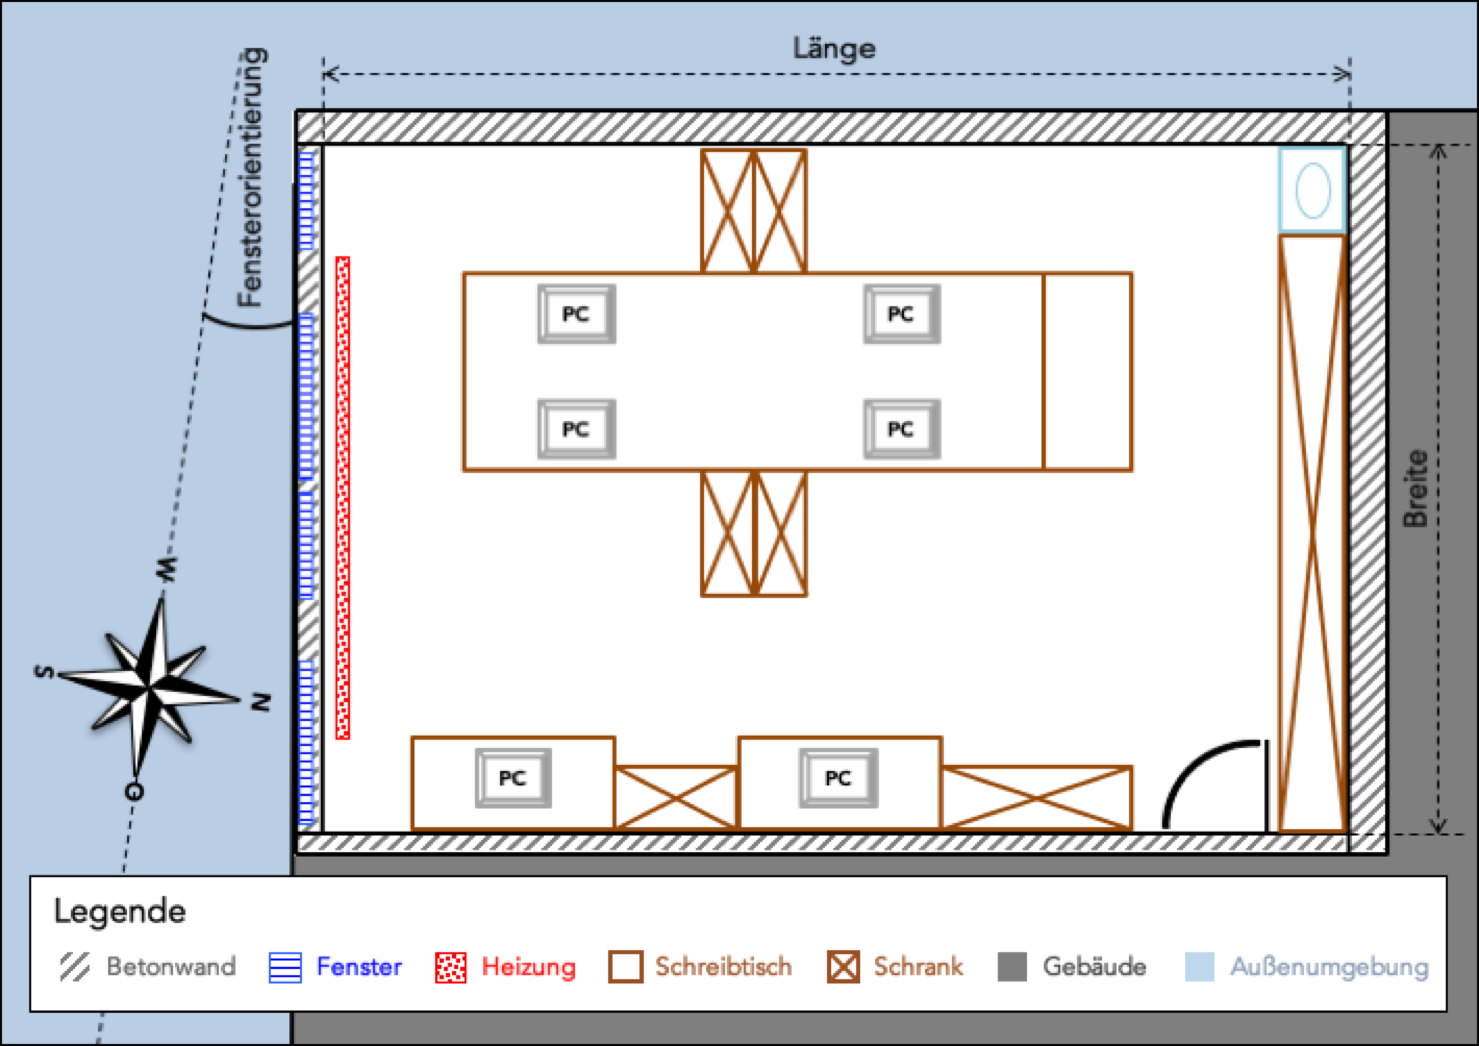
\includegraphics[width=\textwidth]{abbildungen/20160102_k004a}
\caption[Raumskizze K004A vom K Gebäude der Hochschule Karlsruhe -- Technik und Wirtschaft]{Raumskizze K004A vom K Gebäude der Hochschule Karlsruhe -- Technik und Wirtschaft}
\label{fig:skizzek004a}
\end{figure}

\section{Konzipierung der Steuerung}
Die Steuerung der Anlage 
Für die Berechnung von Optimalsteuerungsplänen wird 
Die Optimalsteuerung stellt in diesem Fall den begrenzenden Faktor dar, da die Optimierungsumgebund CasADi für dynamische Systeme nur unter JModelica.org läuft. Daher wird darauf aufbauend das benötigte Modell für die MPC in Modelica gebildet unter Berücksichtigung der Restriktionen bezüglich JModelica. Die gemeinsame Schnittstelle beider ist Python, übder die damit auch die Kommunikation mit den Hardwarekomponenten der Heizungstseurung erfolgen muss/soll.

Bild Hardware ---- Software   Interface Python, da Software darauf angewiesen ist.



Das Hauptaugenmerk bei der Planung liegt deshalb auf der Kompabilität und möglichst großen Einfachheit der einzlenen Komponenten der Heizungstseuerung. 

Die Optimalsteuerung stellt in diesem Fall den begrenzenden Faktor dar, da die Optimierungsumgebund CasADi für dynamische Systeme nur unter JModelica.org läuft. Daher wird darauf aufbauend das benötigte Modell für die MPC in Modelica gebildet unter Berücksichtigung der Restriktionen bezüglich JModelica. Die gemeinsame Schnittstelle beider ist Python, übder die damit auch die Kommunikation mit den Hardwarekomponenten der Heizungstseurung erfolgen muss/soll.

Bild Hardware ---- Software   Interface Python, da Software darauf angewiesen ist.

\section{Umsetzung der Anlage}


\section{Inbetriebnahme und Ansteuerung der Anlage}
